% PREAMBULE
% !BIB TS-program = biber
% !TEX TS-program = xelatexmk
% ITEX TS-program = latex
% !TEX spellcheck = French

\documentclass[class=article, crop=false]{standalone}
\usepackage[subpreambles=true]{standalone}
\usepackage{import}
\usepackage{blindtext}
\usepackage{fontspec}
\usepackage[french]{babel}
\usepackage{caption}
\usepackage{subcaption}
\usepackage{csquotes}
\usepackage{url}

%%%%%%%%%%%%%%%%%%%%%%%%
%			REFERENCES
% le package hyperref avec des options, si en local
\usepackage{hyperref}
\usepackage[backend=bibtex, sorting=nyt, style=verbose-ibid]{biblatex}
\addbibresource{../../../bib.bib}

%%%%%%%%%%%%%%%%%%%%%%%%
%			GLOSSAIRE
\usepackage[acronym]{glossaries}
\makeglossaries
\newglossaryentry{htr}
{
    name=Handwritten Text Recognition,
    description={La reconnaissance du texte écrit sur une image numérique}
}
\newacronym{HTR}{HTR}{Handwritten Text Recognition}

\newglossaryentry{ocr}
{
    name=Optical Character Recognition,
    description={La reconnaissance des polices du texte sur une image numérique}
}
\newacronym{OCR}{OCR}{Optical Character Recognition}

\newglossaryentry{Inria}
{
    name=Inria,
    description={Institut national de recherche en sciences et technologies du numérique}
}
\newacronym{INRIA}{Inria}{Institut national de recherche en sciences et technologies du numérique}

\newglossaryentry{enc}
{
    name=École nationale des chartes,
    description={Grande école bla bla bla}
}
\newacronym{ENC}{ENC}{École nationale des chartes}

\newglossaryentry{HTR-United}
{
    name=HTR-United,
    description={HTR-United is a catalog and an ecosystem for sharing and finding ground truth for optical character or handwritten text recognition (OCR/HTR)}
}

\newglossaryentry{CLab}
{
	name=CREMMALab,
	description={Consortium pour la reconnaissance
d’'écriture manuscrite des matériaux anciens}
}
\newacronym{CREMMA}{CREMMA}{Consortium Reconnaissance
d’Écriture Manuscrite des Matériaux Anciens}

\newglossaryentry{tei}
{
	name={Text Encoding Initiative},
	description={Normes internationales de l'encodage des documents texts}
}
\newacronym{TEI}{TEI}{Text Encoding Initiative}

\newglossaryentry{iiif}
{
	name={International Image Interoperability Framework},
	description={Normes internationales de l'exploitation des images numériques et de leurs métadonnées par API}
}
\newacronym{IIIF}{IIIF}{International Image Interoperability Framework}

\newacronym{ALTO}{ALTO}{Analyzed Layout and Text Object}
\newacronym{XML}{XML}{eXtensible Markup Language}
\newacronym{BNF}{BnF}{Bibliothèque nationale de France}
\newacronym{almanach}{ALMAnaCH}{Automatic Language Modelling and Analysis \& Computational Humanities}
\newacronym{RDF}{RDF}{Resource Description Framework}
\newacronym{TAL}{TAL}{Traitement automatique des langues}


\begin{document}
Le projet \textit{Gallic(orpor)a} s'est développé à partir de plusieurs projets précédents et il tire parti de divers domaines de recherche. Ses créateurs, en mettant en valeur leurs propres connaissances, ont visé à assembler un pipeline qui peut traiter tout document dans la base de données Gallica de la \acrlong{BNF} (\acrshort{BNF}). Les chercheurs spécialisés en \textit{l'\acrlong{HTR}} (\acrshort{HTR}), en le \acrlong{TAL} (\acrshort{TAL}), en l'histoire, en la littérature, en la lexicographie et en la stylométrie se sont rassemblés pour réaliser ce pipeline. Le pipeline visait à prédire et analyser du ancien français et du français de l'Ancien Régime, ainsi que les manuscrits et les imprimés, à partir des pages numérisées des documents créés entre 1400 et la révolution française. Cependant, le vrai rêve du projet était de produire un prototype qui servirait d'exemple et pourrait être élaboré dans le but de traiter vraiment tout document source numérisé.

Les ambitions du \textit{Gallic(orpor)a} se sont rendu possibles grâce aux recherches de plusieurs chercheurs et ingénieurs, tel que Laurent Romary, Philippe Gambette, Thibault Clérice, Pedro Suarez Ortiz, Claire Jahan, Caroline Corbières, et Alexandre Bartz. Mais les principaux qui se chargeaient de la surveillance du projet \textit{Gallic(orpor)a} lors de mon stage en 2022 étaient Jean-Baptiste Camps, Simon Gabay, et Ariane Pinche, qui ont développé des modèles \acrshort{HTR} pour extraire du texte des document numériques dans la base de données Gallica. Chez \Gls{Inria}, en tant que stagiaire, j'ai aussi travaillé en collaboration avec  Benoît Sagot et Rachel Bawden, qui ont développé des outils d'analyse linguistique du texte extrait. Tous ensemble, ces chercheurs de divers spécialités ont contribué leurs connaissances pour produire un processus du traitement polyvalent.

%%%%%%%%%%%%%%%%%%%%%%%%
%			1. CONTEXTE DU PROJET
\section{Le contexte du projet}

\subsubsection{Bibliothèque nationale de France et le Data Lab}
Le Data Lab s'est mis en place au sein de la \acrlong{BNF} (\acrshort{BNF}) en 2021.\footcite{carlinBnFDataLabService2021} Lors de sa première année, le Data Lab a lancé son premier appel aux projets qui mettent en valeur les fonds et les ressources de l'institution phare patrimoniale. Le projet \textit{Gallic(orpor)a} faisait partie des premiers projets acceptés en 2021, à côté des projets \textit{AUREJ} (Accès Unifié aux REssources de la Jouabilité), \textit{GALLICAENV}, \textit{BUZZ-F}, et \textit{AGODA} (Analyse sémantique et Graphes relationnels pour l’Ouverture et l’étude des Débats à l’Assemblée nationale).\footcite[123]{bibliothequenationaledefranceRapportActivite20212022} Ayant sa candidature retenu, \textit{Gallic(orpora)} profitait du financement du Data Lab de la \acrshort{BNF}. La plupart du travail sur le projet a eu lieu pendant la première moitié de 2022, suite au mis en place du stage et des vacations par Ariane Pinche, Simon Gabay, et Benoît Sagot.

\subsubsection{Inria et l'équipe ALMAnaCH}
\Gls{Inria} est l'\acrlong{INRIA} et il compte plusieurs branches dans le monde. La branche parisienne encadre l'équipe \acrshort{almanach} dont le acronyme veut dire \textit{\acrlong{almanach}}. Au sein d'\acrshort{almanach} s'est développé le meilleur modèle \acrshort{TAL} pour la langue française, CamemBERT.\footcite{martinCamemBERTTastyFrench2020} L'équipe \acrshort{almanach} encadre les chercheurs, les ingénieurs, les doctorants, et les stagiaires attachés aux projets concernés soit par le traitement automatique des langues, soit par les humanités numériques. L'acronyme du nom fait référence à ces deux pôles de recherche~: \textit{Automatic Language Modelling and Analysis} est le traitement automatique des langues, et le \textit{Computational Humanities} est l'humanités numériques. Le projet \textit{Gallic(orpor)a} se situait entre les deux, impliquant l'extraction des données et l'édition des documents historiques ainsi que l'analyse linguistique du texte extrait. 

Le directeur de recherches d'\acrshort{almanach} est Benoît Sagot, qui s'est chargé de l'encadrement du stage du projet \textit{Gallic(orpor)a}. En tant que stagiaire, je faisais partie de l'équipe entre début avril et fin juillet 2022. Pendant le stage, Rachel Bawden a animé un groupe de lecture hebdomadaire et des séminaires mensuelles dont j'ai profité dans l'intérêt de me tenir au courant sur les nouvelles recherches et les nouveaux enjeux du \acrshort{TAL}. Elle a aussi développé un modèle \acrshort{TAL} pour le projet \textit{Gallic(orpor)a} et m'a instruit dans sa mise en œuvre.\footcite{bawdenAutomaticNormalisationEarly2022, gabayFreEMcorporaFreEMnormFreEM2022} Disposée d'un bureau, j'ai travaillé en présentiel quatre jours par semaine, passant un jour toutes les semaines à l'\Gls{enc} pour travailler à côté de l'une des chefs du projet, Ariane Pinche. Chez \Gls{Inria}, j'ai profité de l'expertise de mes collègues de l'équipe \acrshort{almanach}, en particulier Alix Chagué et Hugo Scheithauer. L'équipe entière de \textit{Gallic(orpor)a} a aussi profité des serveurs d'\Gls{Inria}, qui prennaient en charge une partie de la puissance de calcul et du stockage de données pour l'interface graphique \acrshort{HTR} \textit{eScriptorium}.

\subsubsection{École nationale des chartes et l'université de Genève}
En tant qu'une école, contrairement à une équipe de recherche comme \acrshort{almanach}, les rôles de l'\Gls{enc} et l'université de Genève dans le projet \textit{Gallic(orpor)a} concernés l'encadrement des chercheurs qui y ont contribué leurs connaissances. L'\Gls{enc} (\acrshort{ENC}) a aussi donné un lieu de travail, dont j'ai profité un jour par semaine. Ariane Pinche, qui était post-doctorante à l'\acrlong{ENC}, et Simon Gabay, maître-assistant à l'université de Genève, ils ont géré la mise en place du stage et des vacations que la bourse du Data Lab de la \acrshort{BNF} a financés pour 2022. L'\acrshort{ENC} et l'université de Genève les ont soutenu lors de l'encadrement des vacations et du stage.

Gabay, Pinche, et deux autres chercheurs qui étaient attachés à l'\acrlong{ENC} pendant le stage, Jean-Baptiste Camps et Thibault Clérice, ont tous contribué au projet \textit{Gallic(orpor)a}. Gabay et Pinche se sont occupés de l'harmonisation des vérités de terrain produites par l'équipe en reliant toute transcription que les vacataires ont faite dans l'interface graphique \textit{eScriptorium}. Pinche et Clérice ont commencé à utilisé les vérités de terrain des documents médiévaux en entraînant des nouveaux modèles de l'\acrshort{HTR} et de la segmentation.\footcite{clericeYALTAiSegmontoManuscript2022} Par rapport à la segmentation, Jean-Baptiste Camps, Pinche, et Gabay ont développé le syntaxe \textit{SegmOnto} qui servait à harmoniser les vérités de terrain produites pour tout document dans le corpus d'entraînement, y compris les manuscrits et les imprimés.\footcite{gabaySegmOntoCommonVocabulary2021} Bien que chaque chercheur ait ses spécialités, ils ont tous collaboré et la division des aspects du projet n'étaient pas aussi fermes qu'ils n'ont pas profité des idées de l'un et de l'autre.

\section{La portée des données d'entraînement}
\label{veritesDeTerrain}
Le projet \textit{Gallic(orpor)a} visait à développer et mettre en pratique les modèles \acrshort{HTR} pouvant traiter tout document français dans la base de données Gallica crée entre le XIVe siècle et la révolution française. Un corpus des documents sources numérisés ainsi qu'une sélection de leurs pages à transcrire étaient choisis comme les données d'entraînement d'un tel modèle \acrshort{HTR}. Les membres de ce corpus sont détaillés dans le section \ref{data:portee} de l'appendice. Le choix se faisait en pensant à la diversité linguistique et à la diversité du genre. Comme montre la Figure \ref{fig:diversite_genre}, il y avait les manuscrits, les incunables, et les imprimés. De plus, chaque type de document a porté plusieurs genres littéraires, y compris la poésie, le récit, et le traité. Dans le cas des imprimés, il y avait aussi des pièces de théâtre.

\begin{figure}[hbt!]
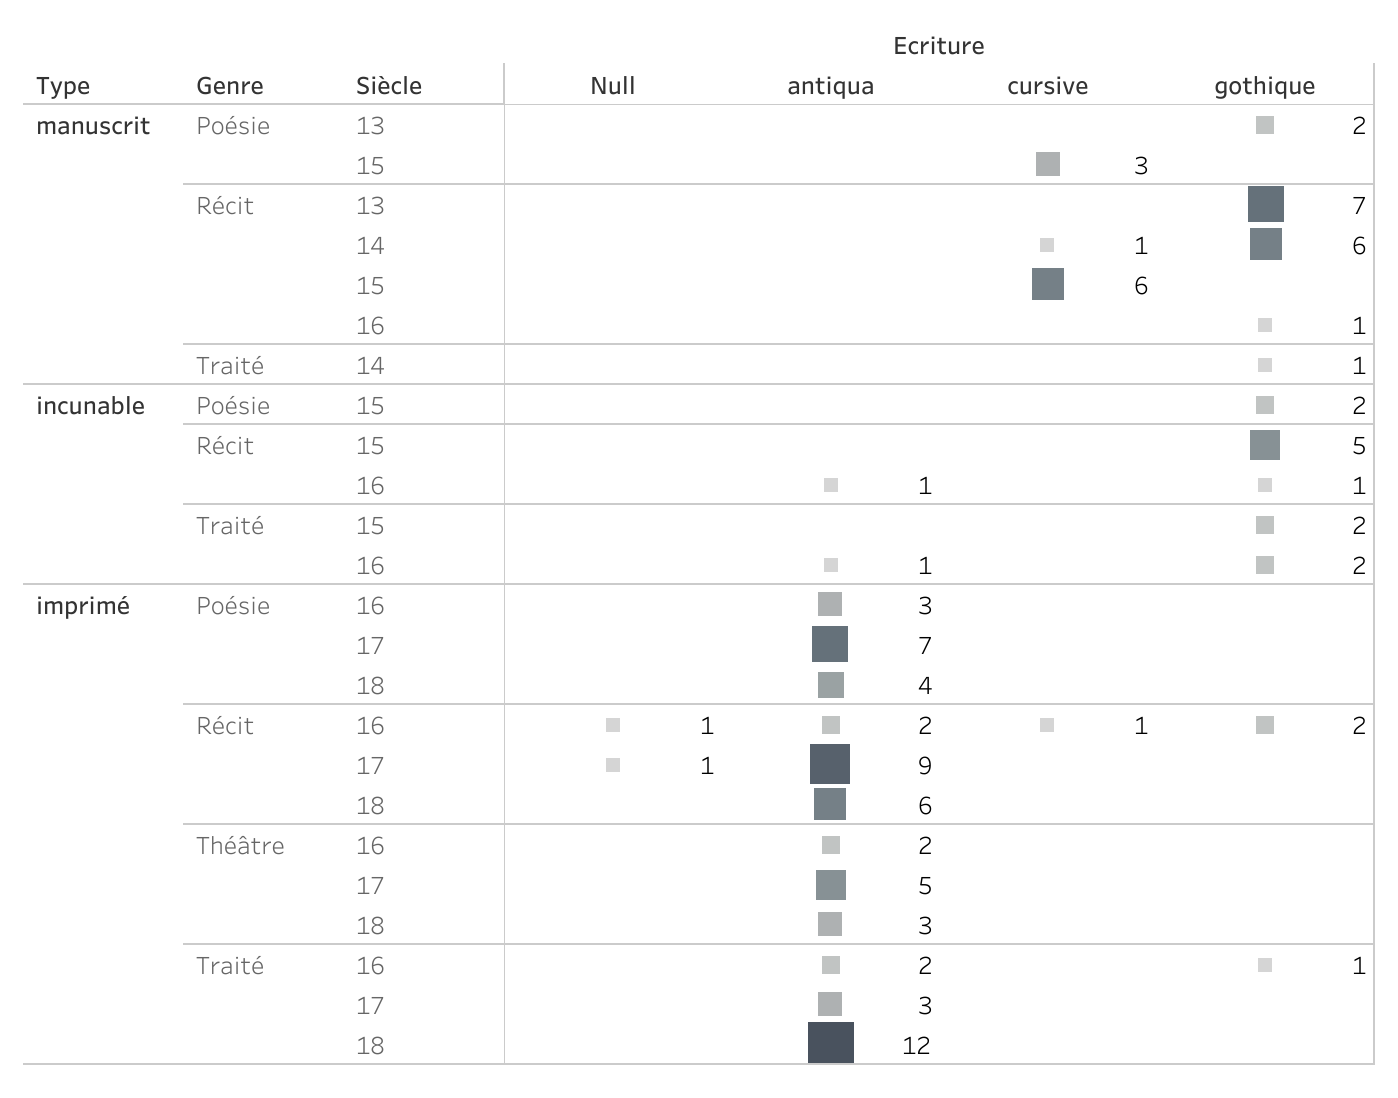
\includegraphics[width=\textwidth]{../../../images/diversite_genre.png}
\caption{Diversité linguistique et générique}
\label{fig:diversite_genre}
\end{figure} 

Pour terminer, un autre souhait quant à la diversité du corpus a porté sur le lieu de publication ou d'apparition du document, comme montre la Figure \ref{fig:diversite_ville}. La plupart des documents choisis de la base de données Gallica étaient sortis de Paris. Une autre partie importante est venue de Lyon. Il y avait aussi un effort d'inclure les manuscrits, les incunables, et les imprimés écrits en français qui sont venus des villes hors de la France, tel que Londres, Amsterdam, et Rome.

\begin{figure}[hbt!]
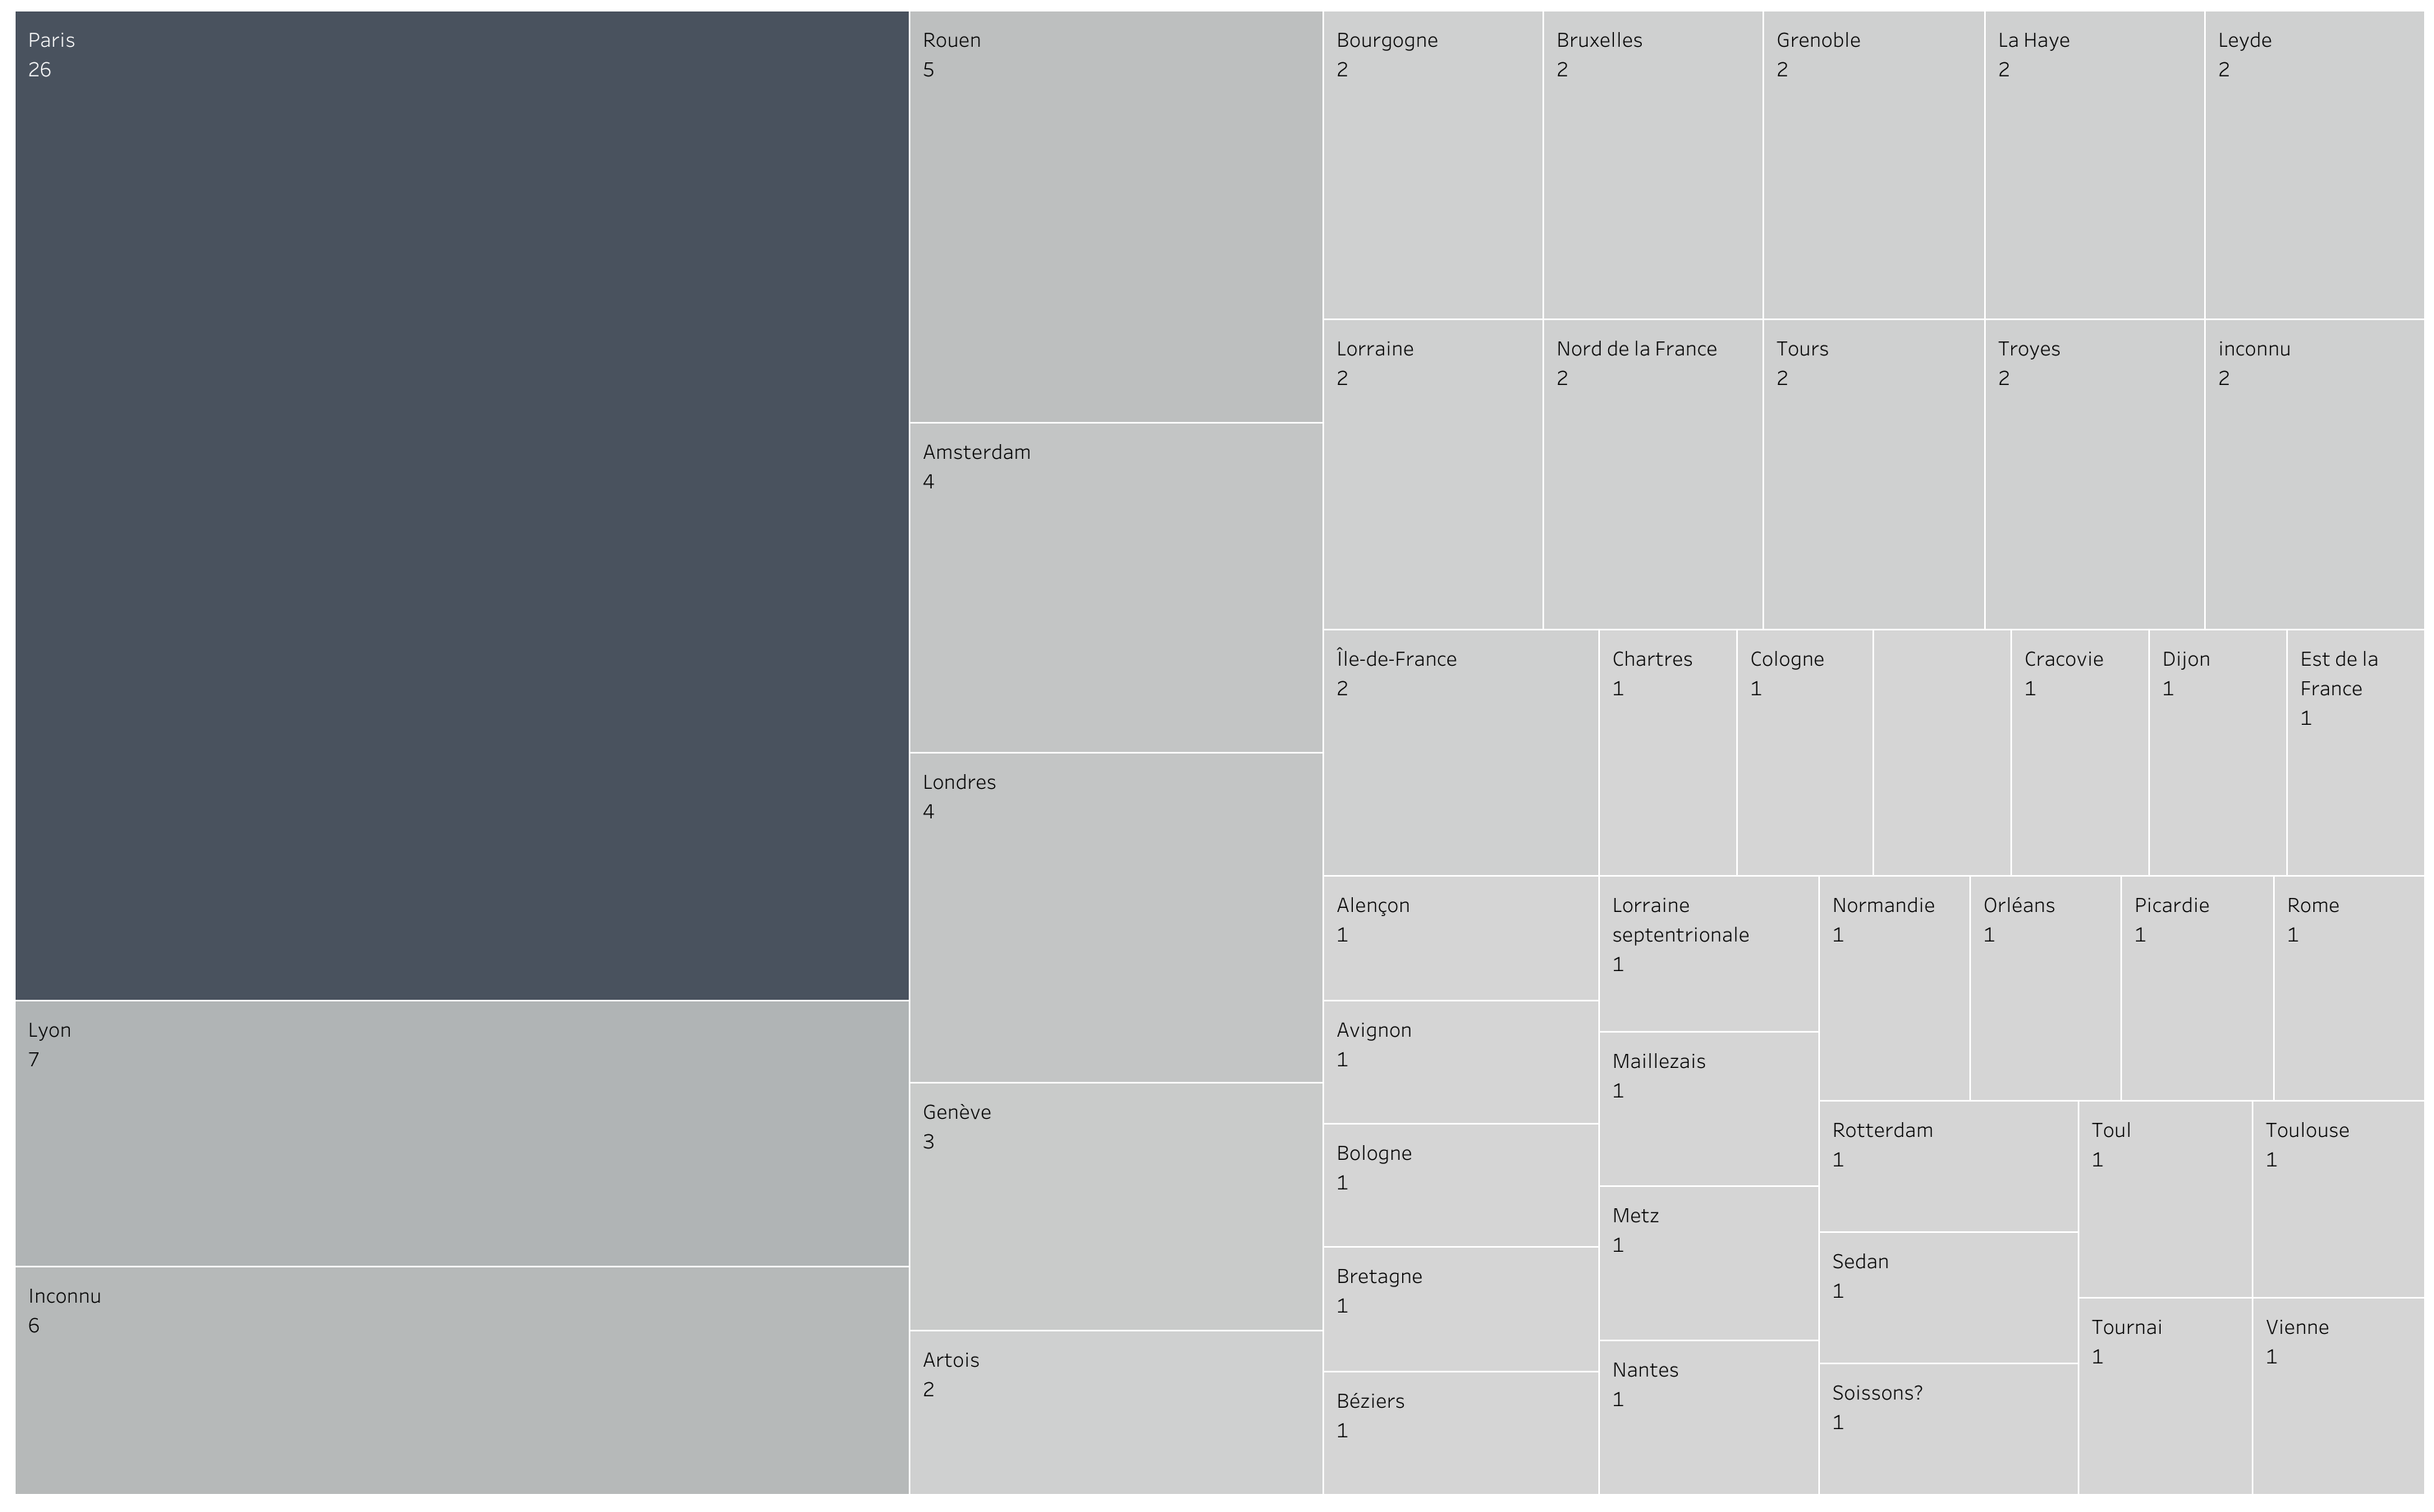
\includegraphics[width=\textwidth]{../../../images/diversite_ville.png}
\caption{Diversité géographique}
\label{fig:diversite_ville}
\end{figure}

Après avoir établi le corpus, les pages ciblées dans chaque document étaient transcrites par des vacataires en utilisant l'interface graphique \textit{eScriptorium}, qui permet à la fois la transcription du texte et la segmentation de la page. La segmentation de la page se faisant en mettant les étiquettes précises sur les masques des lignes et les bloques de texte~; ces étiquettes suivaient le vocabulaire \textit{SegmOnto}. Ensuite, les vérités de terrain produites avec l'interface graphique \textit{eScriptorium} étaient transférées vers les dépôts Github du bon siècle. L'outil \texttt{HTRVX} du projet \Gls{HTR-United} a analysé toute transcription transféré. L'outil s'est alerté aux erreurs potentielles de la segmentation et il a facilité le nettoyage des données.


\section{Les prédécesseurs du projet}
Comme expliqué avant, \textit{Gallic(orpor)a} a rassemblé les recherches de plusieurs projets précédents. Il a profité des glossaires codicologiques, des progrès dans la prédiction et  la segmentation des documents, des progrès dans l'analyse linguistique, et des catalogues des données. Le glossaire \textit{SegmOnto} se servait à harmoniser les vérités de terrain pour les manuscrits et les imprimés transcrits. Les modèles \acrshort{HTR} étaient à la fois un support à la production des vérités de terrain, en faisant en premier temps une transcription préliminaire, et le but du projet, étant de produire les modèles entraînés sur le vocabulaire \textit{SegmOnto}. Le catalogue \Gls{HTR-United}, spécifiquement son outil \texttt{HTRVX}, a surveillé l'harmonisation des transcriptions produites comme des vérités de terrain.\footcite{clericeHTRVXHTRValidation2021} En outre, le catalogue \Gls{HTR-United} a publié gratuitement les vérités de terrain du projet \textit{Gallic(orpor)a} pour que d'autres projets et d'autres modèles \acrshort{HTR} puissent en profiter.\footcite{chagueSharingHTRDatasets2022} Pour terminer, l'analyse linguistique était aussi un objectif du projet \textit{Gallic(orpor)a}, et la mise en œuvre de cet aspect comptait sur les modèles de la langue française construits par les chercheurs de l'équipe \acrshort{almanach}.


\subsubsection{Le glossaire codicologique}
Le projet \textit{Gallic(orpro)a} a harmonisé ses données selon le vocabulaire \textit{SegmOnto}, qui est expliqué en détail dans le chapitre \ref{chap:segmonto}. Ayant géré les données produites selon cette codicologie, j'ai aussi contribué à l'élaboration et le perfectionnement du vocabulaire. La décision d'utiliser le syntaxe descriptif des lignes et des zones de \textit{SegmOnto} a été prise bien en avance de la mise en œuvre du projet \textit{Gallic(orpor)a}. La généralité du vocabulaire était déterminée d'être conforme à la diversité ciblée des documents traités dans le cadre du projet. Puisque \textit{Gallic(orpor)a} visait à livrer un prototype d'un pipeline qui pourrait traiter tout document source numérisé, la généralisation des étiquettes appliquées aux lignes et aux zones était impérative, et le vocabulaire de \textit{SegmOnto} était jugé la meilleure solution.

\subsubsection{La segmentation et la prédiction du texte}
Les progrès de la reconnaissance du texte sont expliqués en détail dans le chapitre \ref{chap:htr}. Un logiciel \acrshort{HTR} commence par la segmentation de la page, et dès qu'il sait où se trouvent les caractères, les mots, et les lignes du texte il le prédit à partir de l'écriture. Ces deux tâches se font selon les compétences qu'il a appris lors de son entraînement. Dans le but de produire les vérités de terrain pouvant entraîner les modèles \acrshort{HTR} pour les manuscrits, les incunables, et les imprimés dans la base de données Gallica, le projet \textit{Gallic(orpor)a} a profité de l'expertise de Simon Gabay et d'Ariane Pinche, qui s'occupaient de la relecture des vérités de terrain et la gestion des corpus d'or.

 Les progrès dans la prédiction du texte sur les imprimés de l'Ancien Régime ainsi que son analyse ont aidé le projet \textit{Gallic(orpor)a}. Par rapport aux progrès dans l'\acrshort{OCR} des imprimés françaises de l'Ancien Régime, Gabay a entraîné les modèles sur les vérités de terrain des imprimés du XVIe au XVIIIe siècle.\footcite{gabayStandardizingLinguisticData2020} En collaboration avec d'autres chercheurs, il a travaillé sur le jeu de données OCR17+ qui a fourni des vérités de terrain des imprimés du XVIIe siècle.\footcite{gabayOCR17GroundTruth2020} Pour tester le pipeline, dans l'attente des modèles nouvellement entraînés sur les données produites dans le cadre de \textit{Gallic(orpor)a}, j'ai utilisé un modèle de segmentation et un modèle d'\acrshort{HTR} que Gabay a développé dans le cadre de son projet \textit{E-ditiones}.\footcite{gabayEditiones17thFrench2018}

Pour la reconnaissance du texte sur les documents médiévaux, le projet \Gls{CLab} est clef. Géré dans le cadre des études postdoctorales d'Ariane Pinche, le \acrlong{CREMMA}, ou \acrshort{CREMMA}, est un dépôt des images et leurs transcriptions corrigées à la main, c'est-à-dire des vérités de terrain. Afin d'entraîner un modèle \acrshort{HTR}, il faut un jeu des vérités de terrain.\footcite{chagueHTRUnitedMutualisonsVerite2021} Le projet \Gls{CLab} fournit un jeu des vérités de terrain de 13 manuscrits médiévaux qui se composent de 21~656 lignes de texte transcrites.\footcite{pincheCremmaLabProjectTranscription2022} Sur les données du projet, Pinche a entraîné un modèle \acrshort{HTR} qui est désormais disponible sur Zenodo.\footcite{pincheHTRModelCremma2022} Le projet \textit{Gallic(orpor)a} en a profité pour aider à la création des vérités de terrain pour les manuscrits médiévaux de son propre jeu de données.

\subsubsection{L'harmonisation et la partage des données}
Le projet \Gls{HTR-United} mis en commun les vérités de terrain générées par tout projet \textit{open source}. \footcite{chagueHTRUnitedHtrunitedV02022} Sa base de données, gratuitement mise en ligne par GitHub, contient les images et leurs transcriptions faites par plusieurs projets de recherche, et elle porte sur les documents de plusieurs périodes historiques et écritures. Un modèle \acrshort{HTR} peut être entraîné sur ces jeux de données. Par exemple, Alix Chagué a entraîné un modèle \acrshort{HTR} sur les vérités de terrain du \textit{LECTAUREP Project}, soutenu par \Gls{Inria} et les Archives Nationales, qui sont mis en commun sur la base de données \Gls{HTR-United}.\footcite{chagueLECTAUREPContemporaryFrench2022}

Dans l'esprit de la science ouverte, le projet \textit{Gallic(orpor)a} a transféré toute vérité de terrain de ses dépôts GitHub vers le catalogue \Gls{HTR-United}. À la fin du stage, en juillet 2022, Ariane Pinche et Thibault Clérice ont entraîné un modèle pour les manuscrits médiévaux en utilisant les transcriptions que l'équipe du projet \textit{Gallic(orpor)a} ont produites. Ces vérités de terrain sont désormais mises en commun sur \Gls{HTR-United} et Pinche et Clérice ont lié le premier modèle publié du projet \textit{Gallic(orpor)a} avec le catalogue \Gls{HTR-United} et le dépot du projet \acrshort{CREMMA} (\acrlong{CREMMA}).\footcite{pincheHTRUnitedCremmamedievalCortado2022} La partage des données du projet est l'un de ses objectifs.

Ainsi qu'à contribuer au catalogue, le projet \textit{Gallic(orpor)a} a aussi profité des outils de \Gls{HTR-United}. Le dernier met en commun des outils qui ont pour but d'harmoniser les données ajoutés à son catalogue. Ces outils peuvent être intégrés dans un \textit{workflow} de GitHub, ce que l'équipe de \textit{Gallic(orpor)a} a fait. L'un de ces outils est \texttt{HTRVX}, qui se prononce comme le personnage Asterix, et il a rendu possible à l'équipe du projet nettoyer les transcriptions sorties de \textit{eScriptorium}.\footcite{clericeHTRVXHTRValidation2021} En exemple, \texttt{HTRVX} relit les transcriptions et les cherche pour les erreurs communes. L'existence d'un tel outil et sa disponibilité gratuite grâce au projet \Gls{HTR-United} a beaucoup aidé le projet \textit{Gallic(orpor)a}.

\subsubsection{L'analyse linguistique}
Après l'extraction et le nettoyage des données des documents source de Gallica, le projet \textit{Gallic(orpor)a} a envisagé à analyser le texte. Dans cet objectif, il a profité des progrès dans l'analyse linguistique des anciens états de la langue française. L'analyse linguistique du français de l'Ancien Régime, tel que ce qui se voit dans les écrits de Molière, est un domaine de recherche actuellement en plein développement. Depuis une dizaine d'années, les chercheurs dans la linguistique computationnelle ont élaboré des outils pour analyser le français autre que le français contemporaine, dont les recherches sont déjà animées par l'application commerciale et les jeux de données plus nombreuses.

L'histoire de l'analyse linguistique et du \acrlong{TAL} (\acrshort{TAL}) est hors de ce mémoire. Néanmoins, les projets qui ont précédés \textit{Gallic(orpor)a} et sur lesquels il a compté méritent de discussion. Achim Stein a bordé le sujet de l'analyse linguistique du français du Moyen Âge dans son article de 2013.\footcite{steinSyntacticAnnotationMedieval2013} Stein a montré que, pour les chercheurs qui ont débuté d'appliquer les progrès dans l'analyse linguistique à l'étude du français des anciens états, il faut faire attention aux propriétés syntaxiques et morphologiques propres à la langue. Du coup, une architecture qui pourrait parvenir aux résultats souhaités pour l'anglais du Moyen Âge n'aura pas forcement le même taux de réussite avec le français du Moyen Âge à cause de différences syntactiques et morphologiques dans la langue.

Achim Stein et Sophie Prévost ont créé un \textit{treebank} pour l'ancien français, le \textit{Syntactic Reference Corpus of Medieval French} (SRCMF), qui avance toujours l'analyse linguistique des anciens états du français.\footcite{steinSyntacticReferenceCorpus2013} En 2014, Prévost est des autres chercheurs, Gael Guibon, Isabelle Tellier, Matthieu Constant, et Kim Gerdes, ont ajouté aux conclusions de Stein que la variation lexique de l'ancien français pose aussi un défi à l'analyse linguistique.\footcite{guibonParsingPoorlyStandardized2014} En 2019, Mathilde Regnault, Prévost, et Éric Villemonte de La Clergerie ont utilisé le SRCMF avec le MCVF (Modéliser le changement : les voies du français) pour encore élaborer notre connaissance de l'évolution du français.\footcite{regnaultChallengesLanguageChange2019} Telles études linguistiques ont tourné la terre pour que l'analyse du texte extrait des manuscrits médiévaux et des imprimés historiques puissent voir le jour aujourd'hui.

\textit{Gallic(orpor)a} a profité des progrès dans l'analyse linguistique du français historique utilisé dans les imprimés et les manuscrits de ses corpus. Jean-Baptiste Camps, Simon Gabay, Paul Fièvre, Thibault Clérice, et Florian Cafiero ont créé \textit{Deucalion} qui est un modèle \acrshort{TAL} pour le français de l'Ancien Régime, entraîné sur les livrets des drames du XVIIe siècle.\footcite{campsCorpusModelsLemmatisation2021} Encore plus récent est le projet \textit{F{\footnotesize RE}EM}qui veut dire \textit{French Early Modern}\footcite{gabayProjetFREEMRessources2022} Dans une présentation du projet à la conférence du Traitement Automatique des Langues Naturelles à Avignon en juin 2022,  les auteurs ont décrit l'un des modèles qu'ils ont développé à partir de l'étude linguistique de l'ancien français.
\begin{displayquote}
L’étude de la langue ne nécessitant pas uniquement un seul outil, mais toute une gamme de solutions, nous avons adopté une approche holistique du problème, en misant sur la création d’un modèle de langue dédié au français d’Ancien Régime, D’AlemBERT\footcite{gabayFreEMAlemBERT2022}, qui devrait venir en soutien des différentes tâches de TAL envisagées.\footcite{gabayProjetFREEMRessources2022} 
\end{displayquote}
Le développement des nouveaux modèles TAL pour les anciens états du français a rendu possible la mise en œuvre d'un tel étape d'analyse au pipeline de \textit{Gallic(orpro)a}.


%%%%%%%%%%%%%%%%%%%%%%%%
%			3. PIPELINE
\section{Le pipeline}
Ainsi que la création des vérités de terrain, qui est expliqué dans la section précédente de ce chapitre (Section \ref{veritesDeTerrain}), le projet \textit{Gallic(orpor)a} avait pour but de créer un pipeline pouvant traiter tout document source de la base de données Gallica. En mettant en œuvre les modèles entraînés, il visait à générer une ressource lexicographique qui porte sur le document source. En commençant par les pages numérisés du document source, la ressource numérique présentera quatre types d'information~:
\begin{enumerate}
\item les métadonnées à propos du document source
\item les données topologiques et linguistiques prédites par \textit{l'\acrlong{HTR}} (\acrshort{HTR})
\item le texte pré-éditorialisé, extrait du document
\item le texte analysé par les outils \acrlong{TAL} (\acrshort{TAL})
\end{enumerate}


Chaque type d'information veut servir une utilité différente que la lectrice éventuelle ou le lecteur éventuel de la ressource pourrait désirer. Les métadonnées s'informent sur trois types de document concerné par le pipeline~: (1) la ressource lexicographique qu'il créé, (2) le fac-similé numérique du document source, (3) le document source physique qui se conserve quelque part, sinon qui a été conservé avant sa disparition. Les données produites par les modèles \acrshort{HTR} présentent la segmentation de la mise en page et la prédiction du texte. Ensuite, le texte pré-éditorialisé est présenté, sans sa segmentation, d'une manière plus convenable à l'analyse linguistique. Et en fin, la ressource présente son analyse du texte prédit grâce à l'application de certains modèles \acrshort{TAL}.

Une visualisation du pipeline se voit dans le Figure~\ref{fig:pipeline}. Elle montre en bleu les saisies des données, en vert les fichiers préliminaires que le pipeline construit, en orange sa première sortie, et en violet les divers moyens d'exploitation de sa sortie. Puisque le pipeline va générer des métadonnées et les données topologiques et linguistiques, il a besoin d'au moins deux saisies des données. L'un porte sur les métadonnées des trois types de document concernés (la ressource lexicographique elle-même, le fac-similé numérique du document source, le document source physique). L'autre saisie des données est l'image numérique elle-même. La première saisie peut se composer de plusieurs sources de données en ligne, afin de fournir à la ressource lexicographique autant de détail que possible. La deuxième saisie se compose du fac-similé numérique dans le format simple des images numériques, tel que JPEG, TIFF, ou PNG.

\begin{figure}[hbt!]
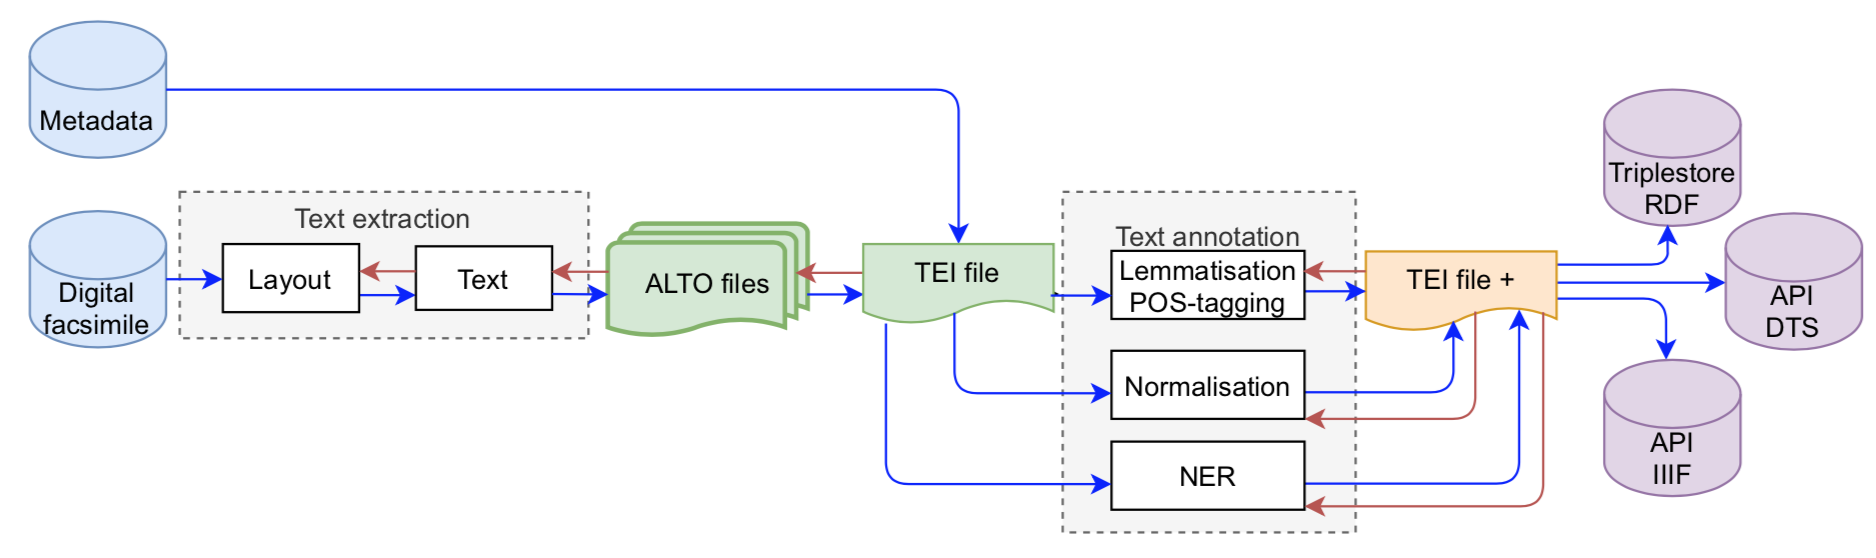
\includegraphics[width=\textwidth]{../../../images/pipeline.png}
\caption{Pipeline}
\label{fig:pipeline}
\end{figure}

En vert, la Figure~\ref{fig:pipeline} montre les premiers fichiers préliminaires créés par le pipeline, les fichiers \acrshort{ALTO}. Ce format d'un fichier \acrshort{XML} est un schéma particulièrement convenable à l'encodage de l'analyse de la mise en page que fait un modèle de segmentation et la prédiction du texte que fait un modèle \acrshort{HTR}. Son acronyme veut dire en anglais \textit{l'\acrlong{ALTO}}, ou la mise en page analysée et l'objet de texte. Comme se voit par la nature bipartite du nom \textit{\acrlong{ALTO}}, les fichiers \acrshort{ALTO} aligne la mise en page et le texte prédit. Le pipeline créé ce genre de fichier préliminaire en appliquant les modèles \acrshort{HTR} aux données d'entrée visuelles.

Après la création des premiers fichiers préliminaires, le pipeline créé la première version du fichier \acrshort{TEI}, qu'il va plus tard enrichir avec l'analyse linguistique du texte prédit. Ce premier fichier \acrshort{TEI} occasionne la création des métadonnées. Comme montre la flèche bleue dans la Figure~\ref{fig:pipeline}, les métadonnées sont récupérées depuis les sources en ligne et ensuite nettoyées et intégrées au fichier \acrshort{TEI}. Le fichier \acrshort{TEI} préliminaire récupère aussi les données des fichiers \acrshort{ALTO}. Il est le combinaison de ces deux genres de données que rend le fichier \acrshort{TEI} bien fait pour présenter toutes les données créés par le pipeline.

À la suite de la récupération, du nettoyage, et enfin de la transformation des données des deux sources pour les conformer au schéma \acrshort{TEI}, le pipeline continue à traiter le texte qu'il a récupéré des fichiers \acrshort{ALTO}. Le pipeline trait deux fois le texte prédit. En premier temps, il parse les données récupérées des fichiers \acrshort{ALTO} et extrait toute ligne de texte imbriquée dans une zone qui fait partie du texte principal. Cela veut dire qu'il n'extrait pas de numéro de page, d'en-tête, etc. Les lignes de texte ainsi sélectionnées sont présentées comme le texte pré-éditorialisé du document source. Elles représentent une espèce de transcription du texte, en ignorant la mise en page et les autres types d'écriture sur la page qui sont communiqués autre part dans le fichier \acrshort{TEI}.

Ce texte pré-éditorialisé peut servir à l'analyse d'une utilisatrice ou d'un utilisateur qui veut appuyer sur le texte tel qu'il était dans le document source. Ce texte sert aussi à la génération d'un texte analysé par les outils \acrshort{TAL}. Le résultat de ce dernier traitement est visualisé dans la Figure~\ref{fig:pipeline} comme la sortie en orange, le fichier \acrshort{TEI} enrichi, \textit{TEI file +}. Pour terminer, les données de la sortie peuvent être exploitées dans plusieurs formats, que la Figure~\ref{fig:pipeline} visualise en violet.

\end{document}
\documentclass[../main.tex]{subfiles}